\subsection{Device}

%\subsection{Design Requirements:}



\textbf{Design Specification}\\

% Table generated by Excel2LaTeX from sheet 'Sheet1'
\begin{table}[htbp]
  \centering
  \caption{Add caption}
\resizebox{\textwidth}{!}{\begin{tabular}{lccll}
\hline
    \multicolumn{1}{c}{No.}&{Requirement} & Wish/Deman & \multicolumn{1}{p{10.785em}}{Importance} & \multicolumn{1}{c}{Engineering Specification}  \\
          &       & \multicolumn{1}{p{8.785em}}{ (1 low, 5 high)} &       &  \\
\hline
1& Sensors open to atmosphere & D & & \\
2&Water Proof & D & & IP67 \\
3&Long battery life & W & 4 & Self powered + battery capacity. > 1 week battery life \\
4&Easy to set up & W & 5 & \\
5&Durable & W & 4 & Sustain accidental drops from height 0.5m \\
6&Low cost & W & 3 & Component and raw material cost < £200 \\
7&Recylable & W & 2 & \\
8&Transparent & W & 4 & \\
9&Easy to charge & W & 2 & Clear acess to charging port \\
10&Cheap to manufacture & W & 3 & Manufacture and assembly cost < £30 \\
11&Small form factor & W & 3 & Overall dimmensions 30x30x30cm \\
\hline
\end{tabular}}%
\label{tab:specification}
\end{table}%

Long Battery Life (4):\\
To ensure regular air quality measurements minimum intervention with the device is required. The most involved element is the charging of the device, therefore this should be kept to a minimum by having a long battery life.
\vskip 0.1in
Easy to set up (5):\\
Crucial to ensuring a citizen science approach to monitoring air quality is maintaining a very simple set up of the sensor. As stipulated in the background the device must be portable and thus require 'packing up' and 'setting up'. Therefore both of these processes must be intuitive (completable without any training or instruction).
\vskip 0.1in
Durable (4):\\
Due to the portable nature of the sensor, and to ensure longevity, the device must be durable to general wear and tear. This has the added benefit of reducing the cost of the air monitoring system by extending the useable life of each sensor.
\vskip 0.1in
Low Cost (3:)\\
In line with the goals of a low cost widely distributed sensor network, the manufacture and component costs must be kept to a minimum to ensure affordability of the device.
\vskip 0.1in
Recyclable (2):\\
In line with responsible use of AI the physical device should not contribute to environmental concerns. This will be achieved by avoiding non-recyclable materials in the design process where possible. These include styrofoam, black plastics and bi-material composites which are hard to separate in the recycling process.
\vskip 0.1in
Transparent (4):\\
The concept of transparent AI can also be extended to the physical device. Ability to view the electronics will demonstrate there are no other devices present such as camera and microphones. An accompanying schematic could be displayed on the website on which the air quality data is displayed. This would detail the components and their purposes in lay terms, which the transparent device would then allow confirmation upon inspection.
\vskip 0.1in
Easy to charge (2):\\
To engage in citizen science effectively, the device should be easy to charge.
\vskip 0.1in
Cheap to manufacture (3):\\
In addition to component cost, the manufacture methods can add considerable cost. Therefore the design should incorporate modularity and simplicity resulting in a minimum number of different manufacturing processes to reduce cost.
\vskip 0.1in
Small form factor (3):\\
The device must be suitable for a variety of different locations, and not take up valuable garden or indoor space.\\
\vskip 0.1in
\textbf{Concepts}\\

A wide variety of concepts were generated using a brainstorming approach. Different design cues and ideas were incorporated into four overall concepts, these are displayed below with key features labelled:


\begin{figure}[H]
\centering
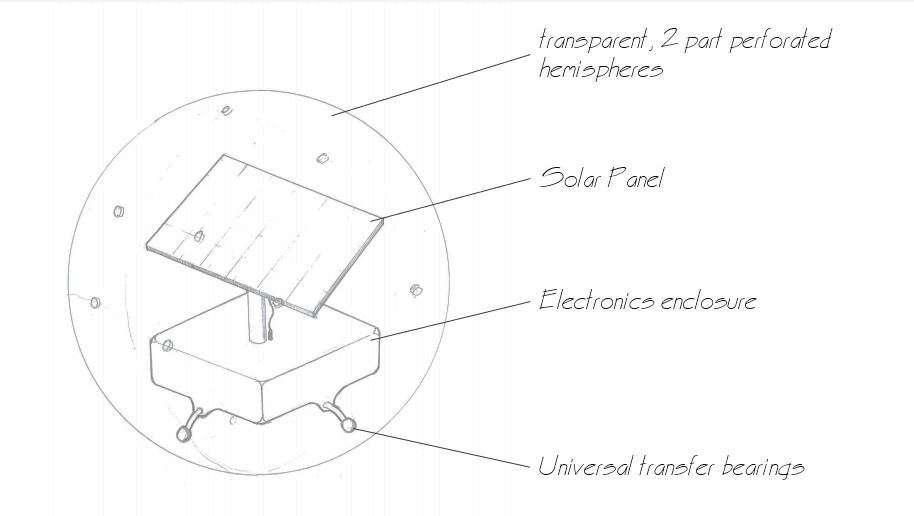
\includegraphics[width=0.6\linewidth]{Engineering_hardware/Engineering_hardware_Figures/Concept_ball.JPG}
\caption{\textbf{Concept A:} A clear sphere surrounds the sensor hardware, the symmetry of the sphere allows the sensors to move within the protective casing. This concept is focused on the specification requirement for easy setup, the self-levelling mechanism ensures a solar panel for charging is always facing up to the light, whilst sensors can be open to the environment and protected from rain by always facing down. }
\label{fig:concept_A}
\end{figure}

\begin{figure}[H]
\centering
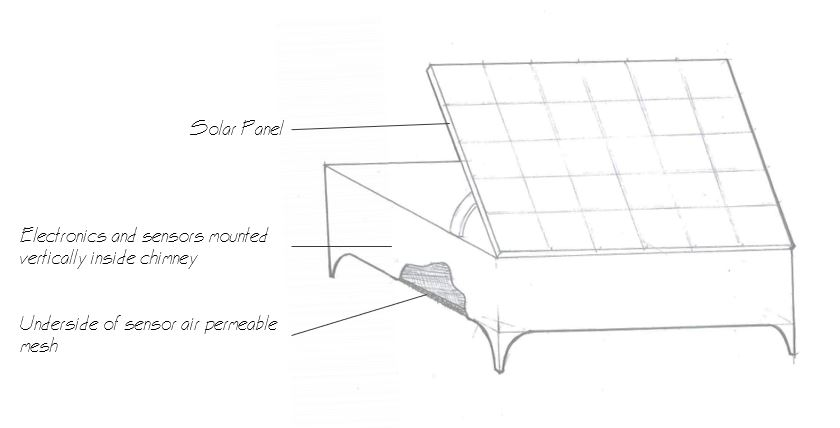
\includegraphics[width=0.6\linewidth]{Engineering_hardware/Engineering_hardware_Figures/Concept_box.JPG}
\caption{\textbf{Concept B:} A solid box contains the sensors, open to the environment and protected from water ingress by a casing raised on small legs. This concept is focused on the specification requirement for low cost; at each stage the design was simplified as much as possible to reduce component cost and simplify the manufacturing and assembly.}
\label{fig:concept_B}
\end{figure}


\begin{figure}[H]
\centering
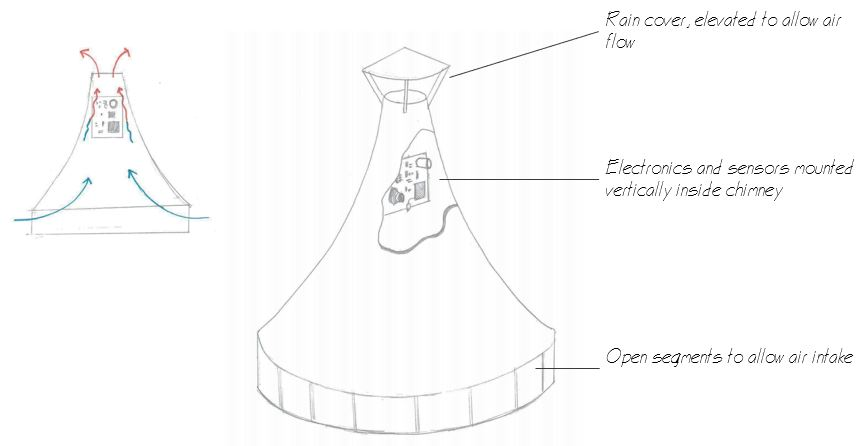
\includegraphics[width=0.6\linewidth]{Engineering_hardware/Engineering_hardware_Figures/Concept_chimney.JPG}
\caption{\textbf{Concept C:} The electronics and sensors are encased in a chimney-like structure. This concept was inspired by using natural convection currents driven by heat given off by the electronics to drive air past the sensors. This solution would be an energy-efficient method for making accurate measurements without the use of an electric fan.}
\label{fig:15cm_shell_loading}
\end{figure}


\begin{figure}[H]
\centering
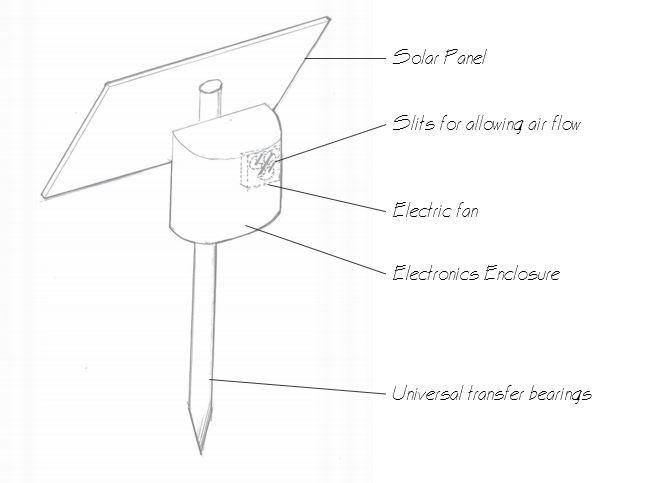
\includegraphics[width=0.6\linewidth]{Engineering_hardware/Engineering_hardware_Figures/Concept_stake.JPG}
\caption{C\textbf{Concept D:} A protective case houses the sensors and electronics, a larger solar panel is used to power an electric fan which feeds air into the sensors. This design is a larger more robust concept of an air quality monitor with a less portable design.}
\label{fig:15cm_shell_loading}
\end{figure}

The four concepts described were then scored against the design criteria specified in table \ref{tab:specification}. The "demand" categories were simple boolean pass-fail criteria. The "wish" categories were given a numeric score 1-5 with five being the best dependant on how well the concept met the specification, this was weighted by the importance of each specification point and summed to give an overall score.

% Table generated by Excel2LaTeX from sheet 'Sheet1'
\begin{table}[htbp]
  \centering
  \caption{Add caption}
    \begin{tabular}{lrrrr}
          & \multicolumn{4}{c}{Concepts} \\
\hline
    Spec No. & \multicolumn{1}{l}{A} & \multicolumn{1}{l}{B} & \multicolumn{1}{l}{C} & \multicolumn{1}{l}{D} \\
\hline
    \multicolumn{1}{r}{1} & 1     & 1     & 1     & 1 \\
    \multicolumn{1}{r}{2} & 1     & 1     & 1     & 1 \\
    \multicolumn{1}{r}{3} & 3     & 5     & 2     & 4 \\
    \multicolumn{1}{r}{4} & 5     & 4     & 3     & 1 \\
    \multicolumn{1}{r}{5} & 5     & 3     & 4     & 3 \\
    \multicolumn{1}{r}{6} & 4     & 5     & 2     & 3 \\
    \multicolumn{1}{r}{7} & 3     & 3     & 3     & 3 \\
    \multicolumn{1}{r}{8} & 5     & 4     & 5     & 3 \\
    \multicolumn{1}{r}{9} & 3     & 5     & 3     & 4 \\
    \multicolumn{1}{r}{10} & 3     & 4     & 2     & 3 \\
    \multicolumn{1}{r}{11} & 4     & 4     & 3     & 2 \\
    weighted sum & \cellcolor[rgb]{ .388,  .745,  .482}127 & \cellcolor[rgb]{ .427,  .757,  .486}126 & \cellcolor[rgb]{ .98,  .616,  .459}96 & \cellcolor[rgb]{ .973,  .412,  .42}86 \\
\hline
    \end{tabular}%
  \label{tab:addlabel}%
\end{table}%

The weighted comparison between concepts revealed that concept A was most suitable for fulfilling the design brief. Prototype B was very close in the overall score however prototype A was perceived to have a few key advantages:
\begin{itemize}
\item A round spherical casing has no localised stress concentrations as opposed to a more angular geometry of prototype B. The sensor would be more robust to impact fractures that it would be exposed to from being dropped.
\item Concept A has a significantly more appealing design in terms of interesting aesthetic and movable internal parts. Although hard to quantify and therefore not included as design criteria, engaging design is more likely to interest the public for citizen science initiatives.
\item The self-levelling design of concept A, although adding some cost ensures the sensor cannot be setup incorrectly, the reliability of readings that this would likely produce is likely to outweigh a small increase in cost.
\end{itemize}

%prototypes for each mechanism:
%locking two parts together


\textbf{Prototype}\\

A prototype was designed and built to test the suitability of the design, the form of the device was designed as a single 3d printed piece. 3d printing is an industry-standard for rapid prototyping, a PLA plastic material was used due to its low melting point and hence high-quality finish. An "off the shelf" Polystyrene, transparent, 180 mm diameter sphere was specified for the casing:
\begin{figure}[H]
\centering
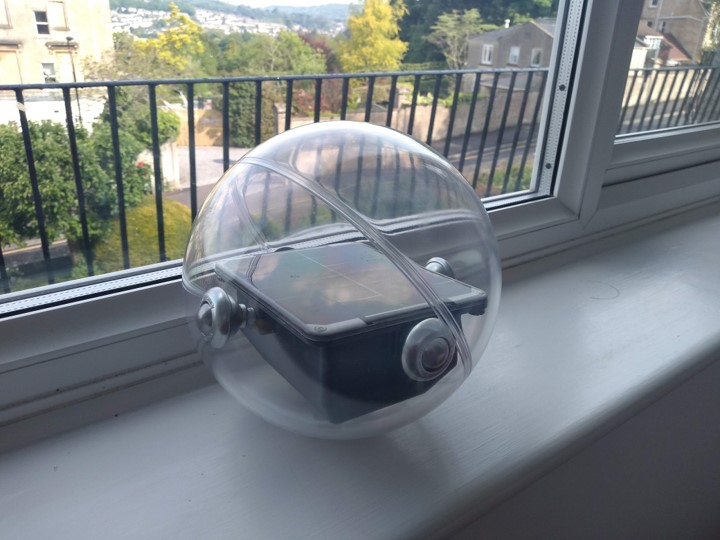
\includegraphics[width=0.5\linewidth]{Engineering_hardware/Engineering_hardware_Figures/airm1.JPG}
\caption{The physical prototype, displayed in a typical setting on a window sill.}
\label{fig:15cm_shell_loading}
\end{figure}

A 6W solar panel was chosen as the maximum surface area that could be accommodated by a device of this size. The prototype included a lithium-ion battery chosen for high capacity compared with size and weight. In addition, a UBEC power converter was used to handle the different voltages from solar panel and battery stepping down to 5V as standard for most small DC electronics including Raspberry Pi single-board computer. 19mm universal bearing were chosen to provide a frictionless interface between the sphere and the electronics casing. A large diameter was chosen to reduce interference between the perforations in the sphere and the movement of the electronics case.

\begin{figure}[H]
\centering
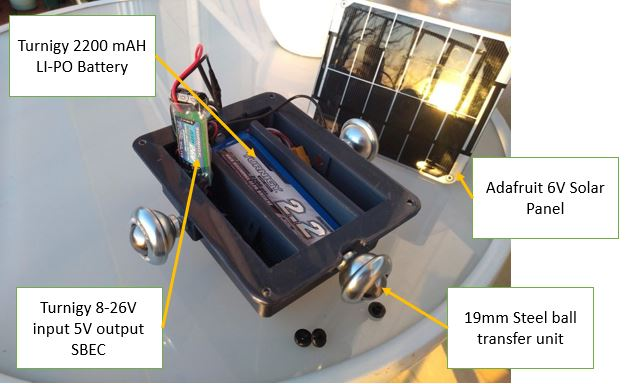
\includegraphics[width=0.5\linewidth]{Engineering_hardware/Engineering_hardware_Figures/prototype_pic_1.JPG}
\caption{Underneath the waterproof solar panel the electronics including battery and power distribution are housed }
\label{fig:15cm_shell_loading}
\end{figure}

A raspberry Pi 3 was used to simulate the custom PCB and sensors developed for this device. The Rasberry Pi runs a Linux operating system which can be interfaced with remotely over WiFi. Power was supplied by a USB-C connection connected to the battery circuitry. The GPIO pins on the Raspberry Pi can be used to interface with other hardware devices. An SGP30 gas sensor was attached to the GPIO pins to produce air quality measurements. To make gas measurements i2c messages were passed to the relevant bus address at a frequency of 1Hz. This was implemented with a Python script run on the Raspberry Pi.

\begin{figure}[H]
\centering
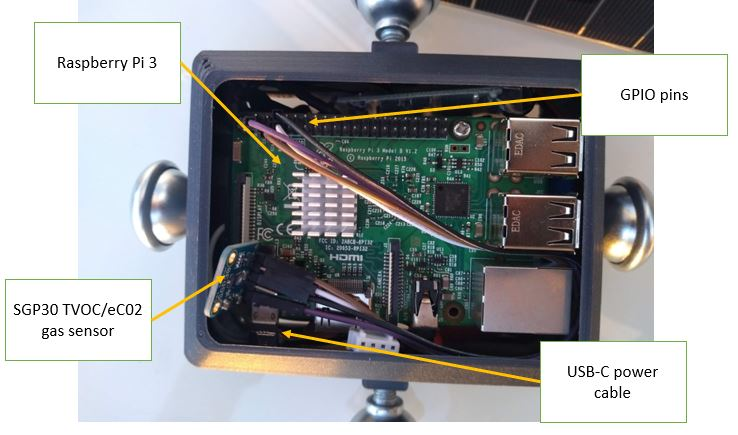
\includegraphics[width=0.5\linewidth]{Engineering_hardware/Engineering_hardware_Figures/prototype_pic_2.JPG}
\caption{The underside of the electronics case is open to the envoronment to allow sensors to measure the air quality.}
\label{fig:15cm_shell_loading}
\end{figure}


%MOVE TO APPENDIX:
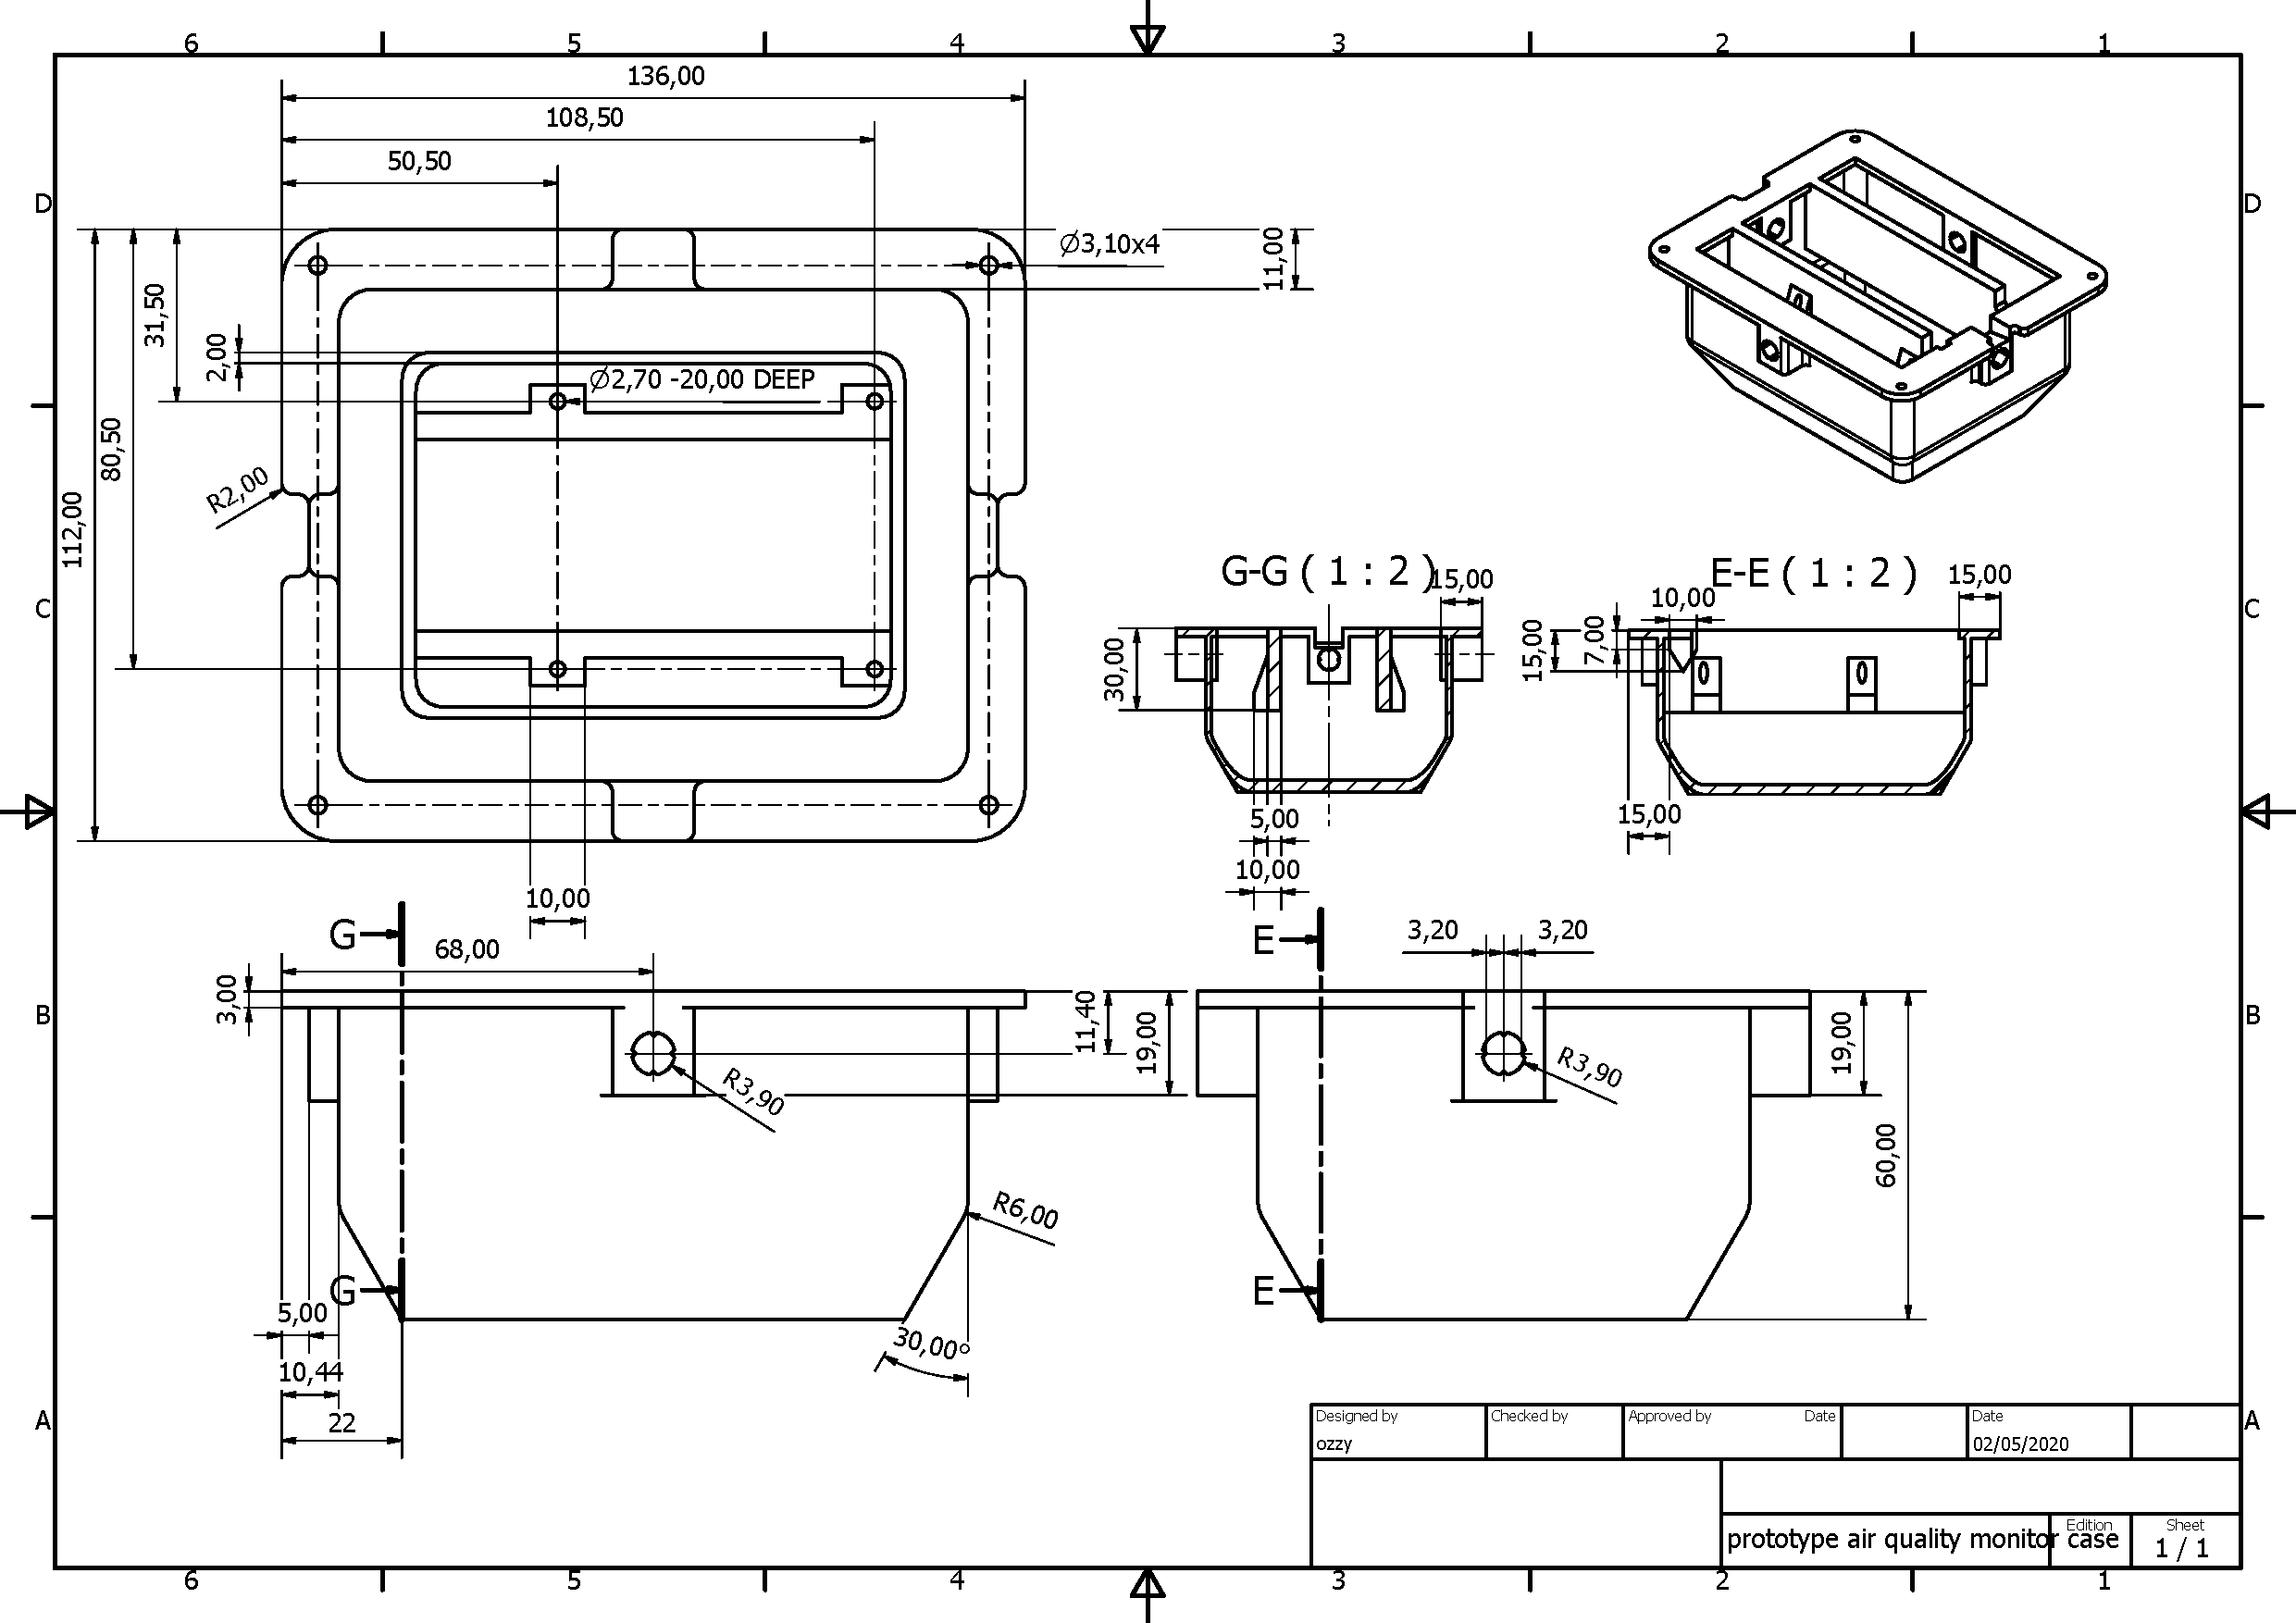
\includepdf[pages={-},fitpaper,rotateoversize]{Engineering_hardware/prototype_air_quality_monitor_case.pdf}

\textbf{Evaluation of prototype:}\\
The prototype provided valuable lessons that influenced the final device design. The need for custom electronics was apparent due to the space requirement of many components and their associated wiring. Additionally, the thickness of the sphere was an important consideration since the weight of the device was sufficient to warp the sphere at the points of applied pressure. This warping was problematic since the universal bearing based design was dependant on equal dimensions along both axes to ensure smooth movement.

It was decided to change the design to use a circular frame attached to the spherical case using ball bearings allowing pivoting along one axis. The electronics case is then attached to the frame perpendicular to the first axis of rotation, and free to pivot using a second pair of ball bearings. As before the electronics case will self-level since the centre of mass is below the pivot point, however, the warping of the sphere will not impede the rotation since it is only in contact at two points.

To design a tolerance that would minimise the size of the device whilst allowing for warping of the spherical case finite element analysis was carried out on the case. The resulting distortion was quantified and a slightly larger tolerance chosen to avoid interference.

\begin{figure}[H]
\centering
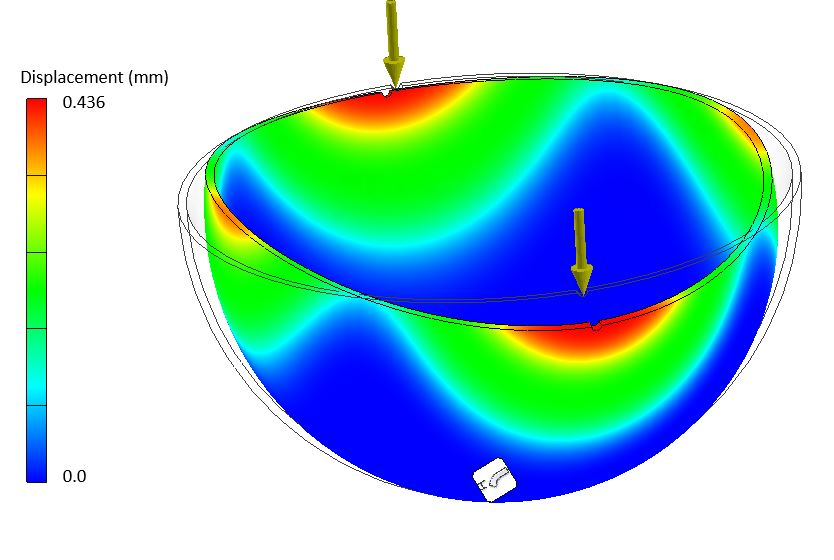
\includegraphics[width=0.5\linewidth]{Engineering_hardware/Engineering_hardware_Figures/FEA.JPG}
\caption{Finite element analysis reveals the extent of deformation experienced under loading from the device mass. This was used to define the tolerence of the self-levelling frame to avoid inteference.}
\label{fig:15cm_shell_loading}
\end{figure}


\textbf{Final Design}
A prototype design was incrementally improved to produce a final design. This includes a wider use of materials, custom parts and manufacturing techniques not available for a rapidly prototyped design but suitable for cost-effective large scale manufacture. The final design was rendered in a photo-realistic environment to give an impression of the final product:

\begin{figure}[H]
\centering
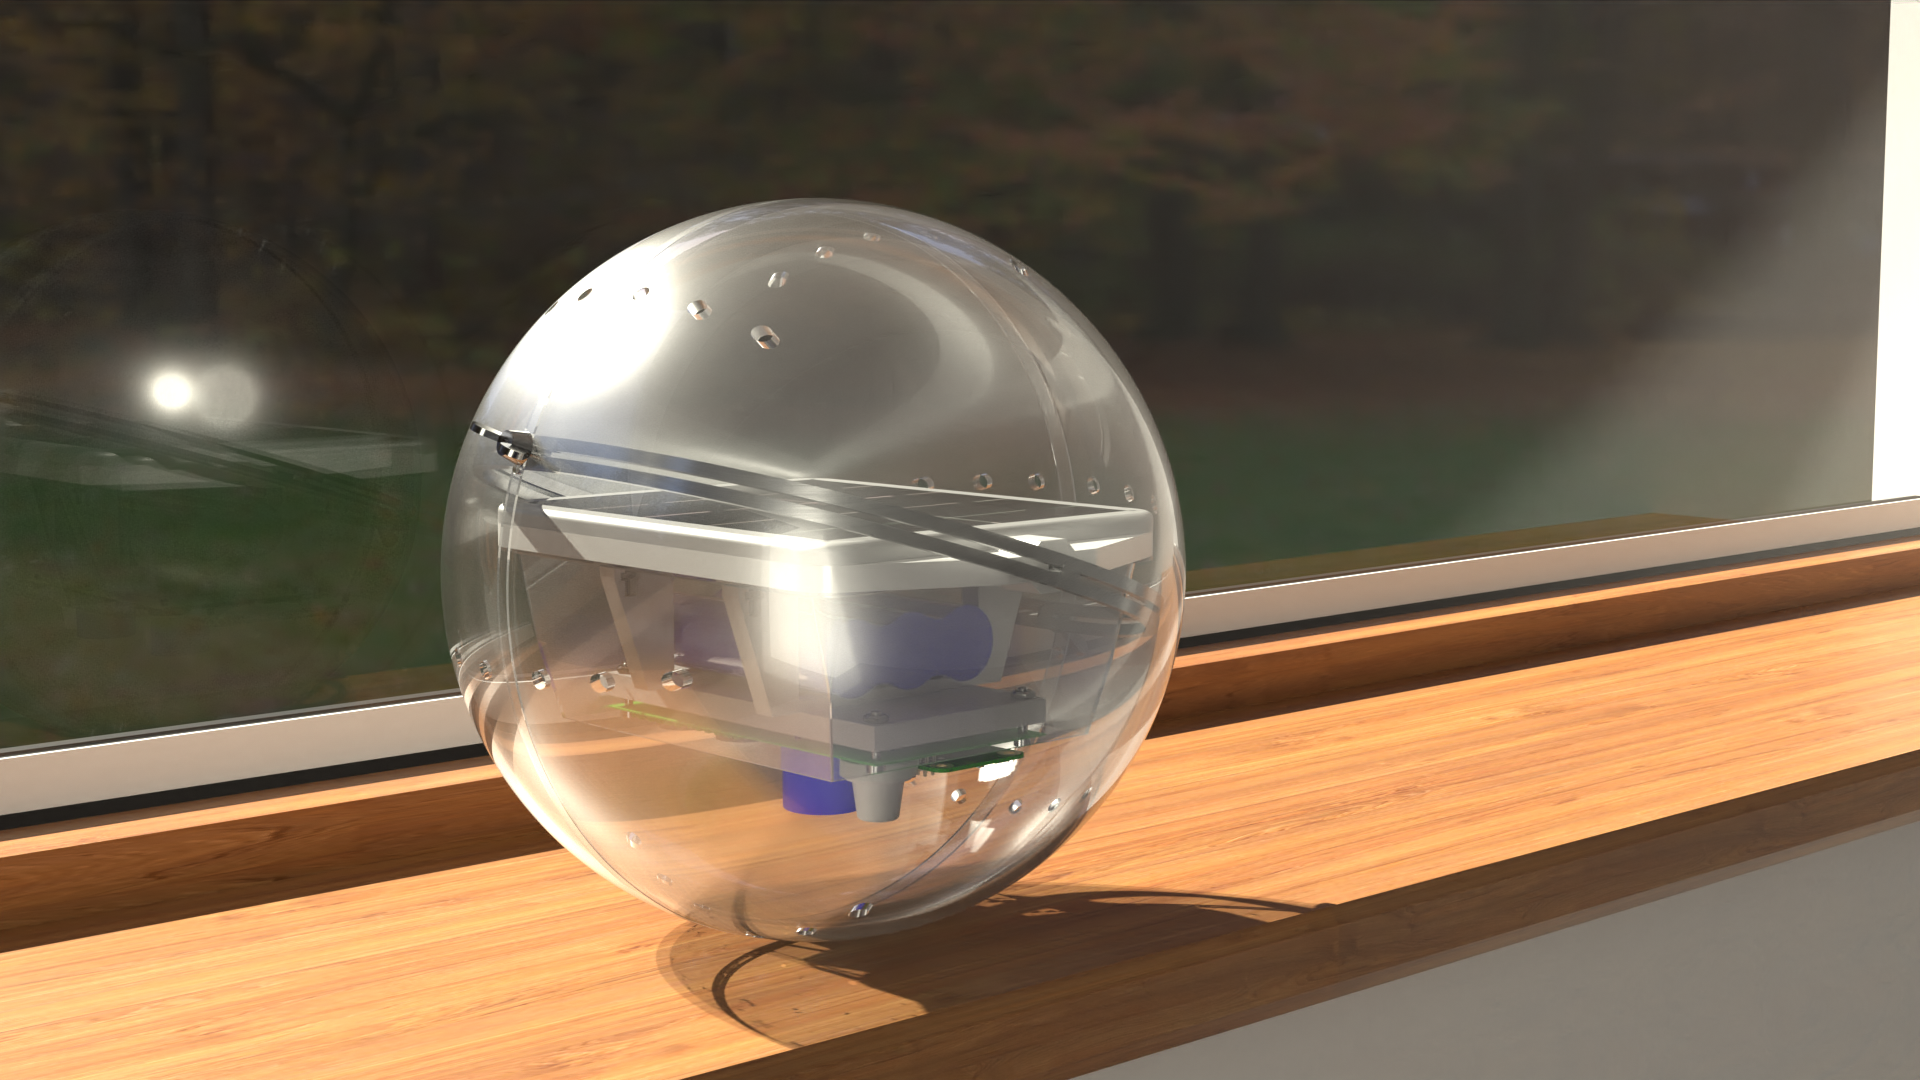
\includegraphics[width=0.8\linewidth]{Engineering_hardware/Engineering_hardware_Figures/0300.png}
\caption{Photo realistic render of the final air quality monitoring device. }
\label{fig:15cm_shell_loading}
\end{figure}
The notable changes from the prototype design are:
\begin{itemize}
\item Mechanism for self-levelling changed to two-axis design.
\item Battery capacity upgraded to 6600mAH
\item Custom PCB for electronics and sensors
\item Electronics casing updated to multiple mass-producible components as opposed to single 3d printed structure.
\end{itemize}
An exploded-view lists all the components that make up the device, and demonstrates the hierarchy of components into an assembly:

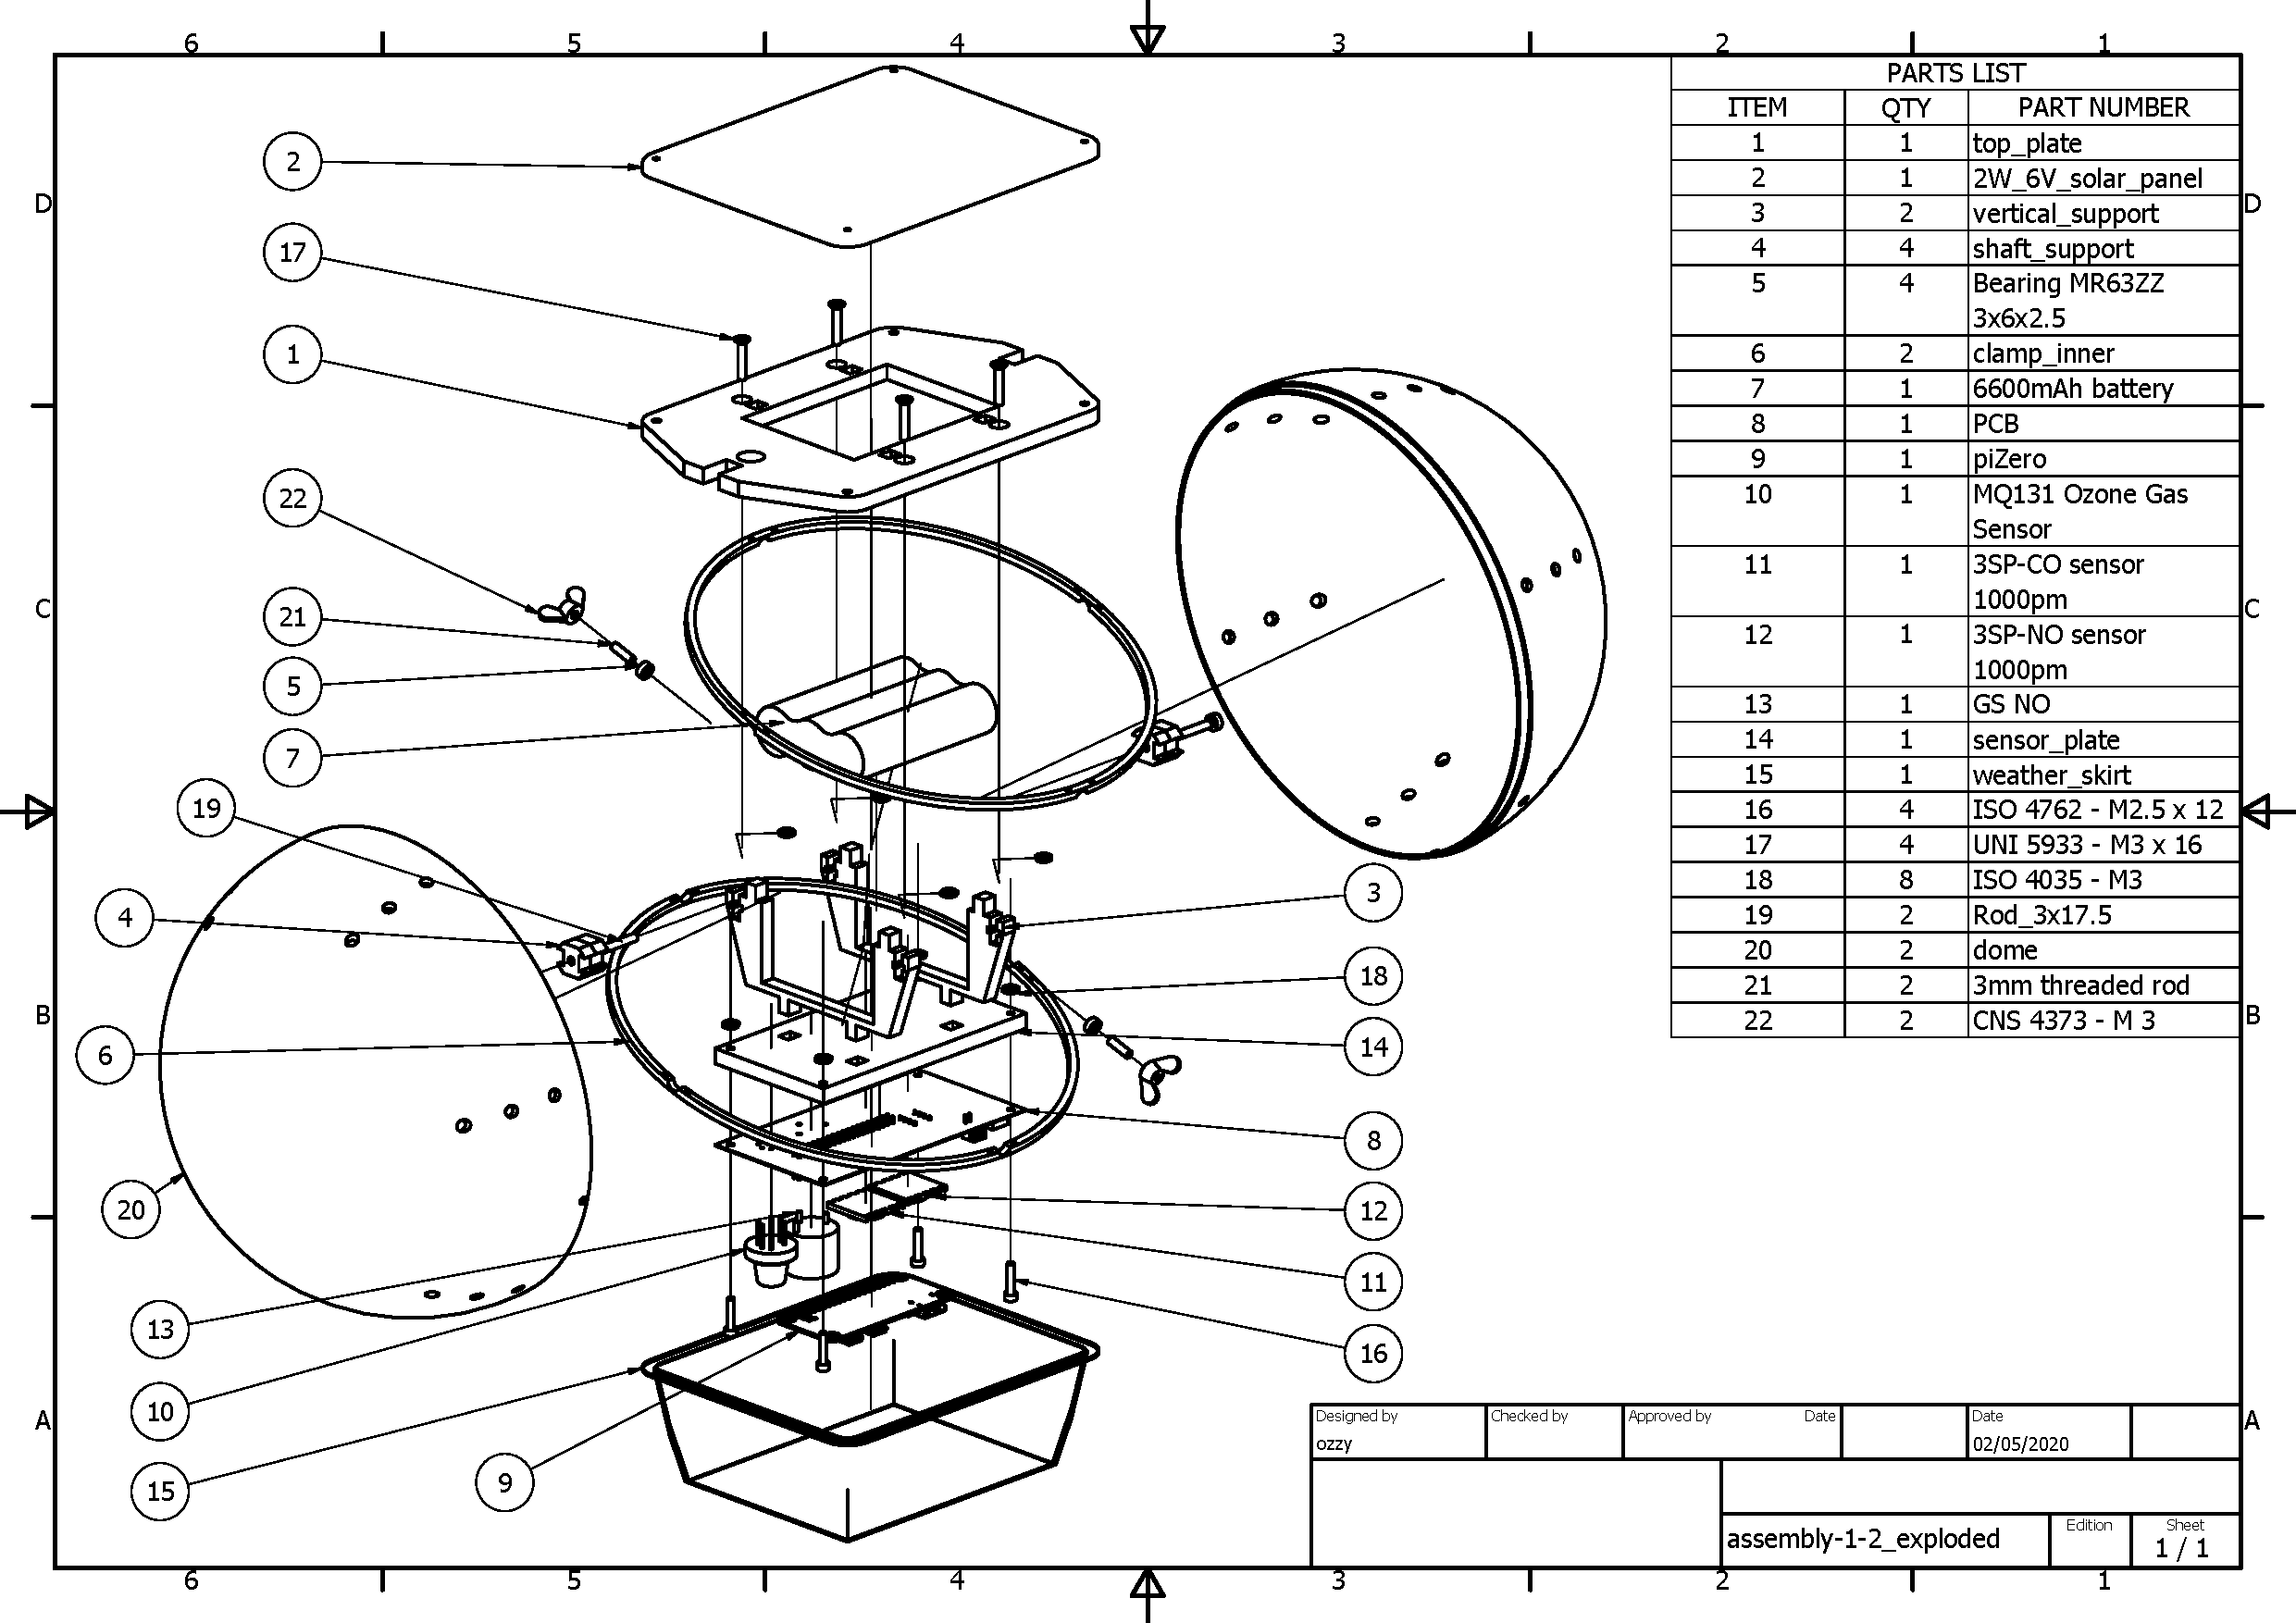
\includepdf[pages={-},fitpaper,rotateoversize]{Engineering_hardware/assembly-1-2_exploded.pdf}

\textbf{Design for Manufacture}\\
The form and material of parts have been carefully considered to provide the required characteristics whilst being mass producible with a simple method for manufacture to reduce cost. Each custom made part has its manufacturing method detailed numbering is per the exploded view:
\begin{itemize}
\item Item 1: Top plate is laser cut from 6mm acrylic. 6mm is a standard thickness of the acrylic sheet, this manufacturing method is very adaptable allowing design changes to be incorporated without any expensive re-tooling. This manufacturing could be easily transferred to injection moulding once sufficient production throughput is required. Post-processing requires countersinking for screw heads, this can be performed by hand or easily automated with a multiheaded attachment to the laser-cutting machine.
\item Item 3: Same as 1.
\item Item 4: Laser cut part (same motivation as part 1) in addition high tolerance of laser-cut part allows for interference fit reducing amount of adhesive required.
\item Item 6: Mild steel was used for the frame as an inexpensive machinable material with sufficient stiffness. The part can be laser cut from steel sheets or cold rolled and welded depending on production capacity required. Anadosing or powder coating would then be applied to produce weatherproofing.
\item Item 14: Same as 1.
\item Item 15: Weather skirt is a non-load bearing transparent part, deep drawing is a suitable manufacturing method for mass-producing moulded thin parts from transparent materials such a polyethylene.
\item Item 20: Dome (two parts), production of this part is likely to be outsourced to a manufacturer specialised in making polystyrene domes. There will be some capital cost for tooling, manufacturing method will be dictated by the supplier but likely to be drawing or vacuum forming, both suitable for mass production.
\end{itemize}


